\chapter{Categorical considerations}
\label{cha:basic-categ-theory}

\renewcommand{\C}{\mathcal{C}}
\newcommand{\D}{\mathcal{D}}

The aim of this chapter is to give a simpler proof of the
\hyperref[th:tellegen]{transposition theorem for arithmetic circuits}
shedding new light on it. The main idea is to bring duality back where
it belongs: category theory. This is done through the use of some
basic categorical semantics~\cite{pitts01,asperti+longo}. We also
discuss the relationship with some Haskell type classes and
perspectives for the implementation of the transposition
principle. This chapter is joint work with Boespflug.



\section{Categorical semantics of arithmetic circuits}
\label{sec:categ-semant-arithm}
\index{categorical~semantics}Categorical semantics introduce the
notion of \index{structure!valued~in~a~category}\emph{structure valued
  in a category $\C$}, which is a generalization of the concept of
\index{structure}\emph{structure} in model theory. This permits to
reason about operations that ``preserve some algebraic structure''.
See~\cite{pitts01} for formal definitions.

Take the example of \index{arithmetic~circuit}arithmetic circuits. In
Section~\ref{sec:circuits} we defined them using left modules and
morphisms, this allowed us to state that the evaluation of a circuit
is a module morphism simply because the composition laws for
arithmetic circuits ``preserve'' the structure. Then in
Section~\ref{sec:multi} we extended the notion of circuit to embrace
circuits containing multiplication nodes; however this meant that we
had to redefine circuits from scratch, considering maps that are not
module morphisms (we did not actually write the new definition in
Section~\ref{sec:multi}, because we were lazy).

The clean way to give both definitions at once, is to consider
\index{arithmetic~circuit!valued~in~a~category}\emph{circuits valued
  in a category $\C$}.  It is soon evident that the only requirement
on the category is that it has finite products; in what follows, we
let $\C$ be a category with finite products.
  
The definition of the syntax of circuits, i.e.\ what are the nodes and
ports, how they are composed to build a circuit, etc., stay the same;
we only change the definitions of operator and of evaluation of an
arithmetic circuit.
  
\begin{definition}[Arithmetic operator, arity]
  Let $A$ be an object of $\C$.  An
  \index{arithmetic~operator}\emph{arithmetic operator} over $A$ is an
  arrow $f:\prod^iA\ra\prod^oA$ for some $i,o\in\N$. Here $i$ is
  called the \index{arity}\emph{in-arity} of $f$ or simply
  \emph{arity}, $o$ is called the \emph{out-arity} of $f$.
\end{definition}
  
\begin{definition}[Evaluation of an arithmetic circuit]
  \index{arithmetic~circuit!semantic}\index{arithmetic~circuit!evaluation}
  Let $A$ be an object of $\C$. Let $C$ be an arithmetic circuit with
  $i$ inputs and $o$ outputs, then its evaluation is an arrow
  $\eval_C:\prod^iA\ra\prod^oA$.
  
  In order to define it, we simultaneously define the evaluation
  $\eval_v$ of each $v\in V$ and the evaluation $\eval_e$ of each
  $e\in E$. We will denote by $<_v$ the orders on the input and the
  output ports of $v$.
  \begin{itemize}
  \item Let $v\in V$ have out-degree $n$, let its evaluation be
    $\eval_v:\prod^iA\ra\prod^nA$ and let $\pi_1,\ldots,\pi_n$ be the
    canonical projections from $\prod^nA$ to $A$. Let
    $o_1<_v\cdots<_vo_n$ be the output ports of $v$ and let
    $e_j=\bigl(o_j,E(o_j)\bigr)$ be the corresponding edges stemming
    from $v$, then $\eval_{e_j} = \pi_j\circ\eval_v$ for any $j$.
  \item Let $x_1<_i\cdots<_ix_i$ be the input nodes and let
    $\pi_1,\ldots,\pi_i$ be the canonical projections from $\prod^iA$
    to $A$, then $\eval_{x_j}=\pi_j$ for any $j$.
  \item For every evaluation node $v$ with in-degree $m$, let
    $i_1<_v\cdots<_vi_m$ be the input ports of $v$ and let
    $e_j=\bigl(E^{-1}(i_j),i_j\bigr)$ be the corresponding edges
    incident to $v$, then
    \begin{equation}
      \eval_v = \beta(v) \circ (\eval_{e_1}\times\cdots\times\eval_{e_m})
      \text{.}
    \end{equation}
  \item For every output node $y$, let $e\in E$ be the only edge
    incident to $y$, then $\eval_y=\eval_e$.
  \end{itemize}
    
  We can finally define $\eval_C:\prod^iA\ra\prod^oA$. Let
  $y_1<_o\cdots<_oy_o$ be the output nodes, then
  \begin{equation}
    \eval_C = \left(\eval_{y_1}\times\cdots\times\eval_{y_o}\right)
    \text{.}
  \end{equation}
  We also say that $C$ \emph{computes} $\eval_C$.
\end{definition}
  
As the reader will have noticed, we have simply taken
Definition~\ref{def:eval} and changed direct sums with categorical
products. Hence, the fact that the evaluation of a circuit in the
category of left modules is a left module morphism is now tautology;
but we can also consider circuits valued in $\mathsf{Set}$, then all
the theory of Section~\ref{sec:multi} can be carried out on those
circuits.
  


\section{Coevaluation}
When dealing with a construction in category theory, it is natural to
simultaneously study its dual, that is the construction obtained by
\emph{reversing all the arrows}. If in definition \ref{def:eval} we
substitute the product $\prod^nR$ by its dual $\coprod^nR$, we obtain
a new way of evaluating an arithmetic circuit that we will call
\emph{coevaluation}. In this section we let $\mathcal{D}$ be a
category with finite coproducts.

An arithmetic cobasis is just an arithmetic basis in $\D^\op$, and the
coevaluation of an arithmetic circuit is just its evaluation in
$\D^\op$. For completeness, we give the detailed definitions.

\begin{definition}[Arithmetic co-operator, arity]
  Let $A$ be an object of $\D$.  An \emph{arithmetic co-operator} over
  $A$ is an arrow $f:\coprod^iA\ra\coprod^oA$ for some $i,o\in\N$.
\end{definition}

\begin{definition}[coevaluation of an arithmetic circuit]
  \label{def:coeval}
  Let $A$ be an object of $\D$.  Let $C$ be an arithmetic circuit with
  $i$ inputs and $o$ outputs over a cobasis $\mathcal{B}$. Its
  coevaluation is an arrow $\lave_C:\coprod^iA\ra\coprod^oA$.

  We use the same notation as in the previous definition. As we did
  there, we simultaneously define $\lave_v$ for each $v\in V$ and
  $\lave_e$ for each $e\in E$.
  \begin{itemize}
  \item Let $v\in V$ have in-degree $m$, let its coevaluation be
    $\lave_v:\coprod^mA\ra\coprod^oA$ and let $\iota_1,\ldots,\iota_n$ be the
    canonical injections from $A$ to $\coprod^mA$. Let $i_1<_v\cdots<_vi_m$
    be the input ports of $v$ and let
    $e_j=\bigl(i_j,E^{-1}(i_j)\bigr)$ be the corresponding edges
    incident to $v$, then $\lave_{e_j} = \lave_v\circ\iota_j$ for any
    $j$.
  \item Let $y_1<_V\cdots<_Vy_n$ be the output nodes and let
    $\iota_1,\ldots,\iota_o$ be the canonical injections from $A$ to
    $\coprod^oA$, then $\lave_{y_j}=\iota_j$ for any $j$.
  \item For every evaluation node $v$ with out-degree $n$, let
    $o_1<_v\cdots<_vo_n$ be the output ports of $v$ and let
    $e_j=\bigl(E(o_j),o_j\bigr)$ be the corresponding edges
    stemming from $v$, then
    \begin{equation}
      \label{eq:lave_v}
      \lave_v = (\lave_{e_1}+\cdots+\lave_{e_n}) \circ \beta(v) 
      \text{.}
    \end{equation}
  \item For every input node $x$, let $e\in E$ be the only edge
    stemming from $x$, then $\lave_x=\lave_e$.
  \end{itemize}

  We can finally define $\lave_C:\coprod^iA\ra\coprod^oA$. Let
  $x_1<_V\cdots<_Vx_i$ be the input nodes, then
  \begin{equation}
    \label{eq:lave}
    \lave_C = \lave_{x_1}+\cdots+\lave_{x_i}
    \text{.}
  \end{equation}
\end{definition}

The coevaluation in general does not attach the same semantics to a
circuit as the evaluation. For example in the case of $\mathsf{Set}$
the coevaluation is a function from the disjoint union of $i$ copies
of $A$ to the disjoint union of $o$ copies of $A$. We can regard
circuits over cobases in $\mathsf{Set}$ as objects that are fed one
single element of $A$ on one out of their $n$ inputs and then take
decisions depending on which input was fed. An example is given in
figure \ref{fig:coffee}.

\begin{figure}[!ht]
  \centering
  
  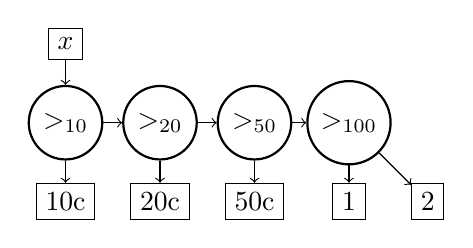
\begin{tikzpicture}
    \tikzstyle{node}=[circle,thick,draw=black,minimum size=4mm]
    \tikzstyle{arg}=[rectangle,thin,draw=black,minimum size=4mm]

    \begin{scope}
      \node[arg](in){$x$};

      \node[node,below of=in](s10){$>_{10}$};

      \node[node,right of=s10,xshift=2mm](s20){$>_{20}$};
      \node[arg,below of=s10](o10){$10$c};

      \node[node,right of=s20,xshift=2mm](s50){$>_{50}$};
      \node[arg,below of=s20](o20){$20$c};

      \node[node,right of=s50,xshift=2mm](s1){$>_{100}$};
      \node[arg,below of=s50](o50){$50$c};

      \node[arg,below of=s1](o1){$1$\euro};
      \node[arg,right of=o1](o2){$2$\euro};

      \path[->]
      (in) edge (s10)
      (s10) edge (o10)
      (s10) edge (s20)
      (s20) edge (o20)
      (s20) edge (s50)
      (s50) edge (o50)
      (s50) edge (s1)
      (s1) edge (o1)
      (s1) edge (o2);
    \end{scope}
  \end{tikzpicture}  
  
  \caption{The coffee machine circuit. On input $n\in\Z$, the operator
    $>_x:\Z\ra\Z\uplus\Z$ gives $n$ on its right output if $n>x$,
    on its left output otherwise. The circuit is an euro coin
    separator.}
  \label{fig:coffee}
\end{figure}

In some cases, howevever, evaluation and coevaluation coincide. Recall
that an \emph{additive category} is a category if every hom-set is an
abelian group, composition of morphisms is bilinear, and every finite
biproduct exists~\cite[VIII.2]{mclane}. In particular, in an additive
category finite products and coproducts are isomorphic.

\begin{lemma}
  \label{th:coeval}
  Let $C$ be a circuit valued in an additive category, then
  $\eval_C\isom\lave_C$ naturally.
\end{lemma}
We just sketch the proof.
\begin{proof}
  First observe that since products and coproducts are naturally
  isomorphic, the basis of $C$ can be interpreted both as a basis and
  a cobasis. Hence both evaluation and coevaluation $C$ are
  meaningful.

  Then, we proceed by induction on the size of the circuit. First, it
  is obvious that for circuits with one unique evaluation node $v$ we
  have $\eval_C\isom\beta(v)\isom\lave_C$. Now if $C$ has $n$
  evaluation nodes, we chose any topological order on $C$ and remove
  the last evaluation node $v$ and the output nodes connected to
  it. This new circuit satisfies the lemma by induction. The claim
  follows by connecting $v$ back to the circuit.
\end{proof}


\section{The tranposition theorem}
\label{sec:tranposition-theorem}
We restate the notion of \hyperref[def:dual]{dual circuit} in our new
context. The dual circuit is obtained by reversing all the arrows, and
it is valued in the opposite category $\C^\op$. Although we use the
same notation, the reader shall not confuse this definition of the
dual circuit $C^\op$ with the definition of the \emph{opposite
  circuit} we gave in Section~\ref{sec:bilinear-chains}.

\begin{definition}[Dual basis]
  Let $A$ be an object of $\C$ and let $\mathcal{B}$ be an arithmetic
  basis over $A$. We define the dual basis $\mathcal{B}^\op$ as
  \begin{equation}
    \mathcal{B}^\op= \{f^\op \,|\, f\in\mathcal{B}\}
    \text{.}
  \end{equation}
\end{definition}

\begin{definition}[Dual circuit]
  \index{arithmetic~circuit!dual} Let $A$ be an object of $\C$. Let
  ${C=(V,E,\le,\le_i,\le_o)}$ be a circuit over $(A,\mathcal{B})$. For
  any $v\in V$ define
  \begin{equation}
    v^\op =
    \begin{cases}
    (O,I,f^\op)              &\text{if $v=(I,O,f)$ with $f\ne\emptyset$,}\\
    (O,\emptyset,\emptyset) &\text{if $v=(\emptyset,O,\emptyset)$,}\\
    (\emptyset,I,\emptyset) &\text{if $v=(I,\emptyset,\emptyset)$.}
    \end{cases}
  \end{equation}

  The \emph{dual circuit} of $C$, denoted by $C^\op$, is the circuit
  over $(A,\mathcal{B}^\op)$ defined as
  \[C^\op = (V^\op, E^{-1},\le^\op,\le_i',\le_o')\text{,}\]
  where $V^\op=\{v^\op|v\in V\}$ and the orderings are defined
  as follows:
  \begin{align}
    v \le v' \;&\Leftrightarrow\; {v'}^\op \le^\op {v}^\op\text{,}\\
    v \le_o v' \;&\Leftrightarrow\; {v}^\op \le_o' {v'}^\op\text{,}\\
    v \le_i v' \;&\Leftrightarrow\; {v}^\op \le_i' {v'}^\op\text{.}
  \end{align}
\end{definition}


We now have all the elements to prove the transposition theorem. We
let $\C$ and $\C'$ be categories with finite products.  The first,
trivial, observation is that certain functors ``preserve'' the
semantic of a circuit. If $F:\C\ra\C'$ is a functor, we define by
$F(\mathcal{B})$ the basis obtained by substituting any arrow $f$ with
$F(f)$ and by $F(C)$ the circuit obtained by substituting any node
with the corresponding node in $F(\mathcal{B})$.

\begin{proposition}
  Let $F:\C\ra\C'$ be a continuous functor (i.e.\ a functor that
  preserves small limits; we actually only need it to preserve
  products). Let $C$ be a circuit valued in $\C$. Then $F(C)$ is
  valued in $\C'$ and $F(\eval_C)=\eval_{F(C)}$.
\end{proposition}

\begin{corollary}
  Let $\C$ be a category with finite products, $\D$ a category with
  finite coproducts and $F:\C\ra\D^\op$ a continuous functor. Then
  $F(C)^\op$ is valued in $\D$ and $F(\eval_C)^\op=\lave_{F(C)^{\op}}$.
\end{corollary}

\begin{corollary}[Transposition theorem]
  Let $\C$ be an additive category and let $F:\C\ra\C^\op$ be a
  continuous functor. Then $F(\eval_{C})^\op\isom\eval_{F(C)^\op}$.
\end{corollary}

The transposition theorem of Section~\ref{sec:tellegen}, then follows
by considering the transposition functor $\dual{()}:R\text{\sf-Mod}\ra
R^\op\text{\sf-Mod}$ (note that the transposition functor is naturally
written in a contravariant fashion).


\section{From circuits to function-level programming}
\label{sec:fp}
\index{arrow}
\lstset{language=haskell} People who think that categories are just
abstract nonsense, may be surprised discovering that arithmetic
circuits valued in $\mathsf{Hask}$ (the category of Haskell types) are
already implemented in Haskell. Alternatively, they might think that
Haskell is concrete nonsense.

The package \lstinline+Control.Arrow+ implements what are commonly
called \emph{arrows} in Haskell jargon. Arrows were introduced in
\cite{hughes98} as a generalization of \emph{monads}, they have been
successfully applied to many different settings such as, for example,
solving ordinary differential equations
\cite{liu+hudak10}. Paterson~\cite{paterson01} was the first to
realize the relationship between circuits and arrows, and to propose a
DSL for arrows that is amazingly similar to straight line programs.

The standard library class \lstinline+Arrow+ is roughly equivalent to
arithmetic circuits valued in $\mathsf{Hask}$ (or $\mathsf{Set}$),
while \lstinline+ArrowChoice+ is roughly equivalent to arithmetic
circuits valued in $\mathsf{Hask}^\op$. So we asked ourselves the
question of whether it is possible to write a type class
\lstinline+AdditiveArrow+ that has the same properties of circuits
valued in additive categories. A desirable feature of \emph{additive
  arrows} is that they could be evaluated both in $\C$ and $\C^\op$,
thus the share some similarities with \emph{invertible
  arrows}~\cite{alimarine+al:invertible-arrows}.

We sketch what an additive arrow should look like, by giving an
hypothetical list of type classes; following
\cite{yorgey:typeclassopedia}, we use infix operators \lstinline+(~>)+
instead of prefix ones as in the standard Haskell library.  As for
arrows, we start from the class \lstinline+Category+.

\begin{lstlisting}
  class Category (~>) => where
    id :: (a ~> a)
    (.) :: (b ~> c) -> (a ~> b) -> (a ~> c)
\end{lstlisting}

In order to behave as a category, an instance of this class shall form
a monoid for the operation \lstinline+(.)+, with \lstinline+id+ being
the identity element. Now this class can be extended to model additive
categories: we first define a class that mimics \emph{Ab-categories},
or \emph{preadditive} categories, that is categories whose hom-sets
are abelian groups, then we define additive categories.

\begin{lstlisting}
  class Category (~>) => AbCategory (~>) where
    zeroArrow :: (a ~> b)
    (<+>) :: (a ~> b) -> (a ~> b) -> (a ~> b)
\end{lstlisting}

\begin{lstlisting}
  class AbCategory (~>) => AdditiveCategory (~>) where
    (&&&) :: (a ~> b) -> (a ~> c) -> (a ~> (b, c))
    (|||) :: (a ~> c) -> (b ~> c) -> ((a, b) ~> c)
    (***) :: (a ~> b) -> (c ~> d) -> ((a, c) ~> (b, d))
\end{lstlisting}

Where \lstinline+&&&+ roughly corresponds to the operator $\hub$ of
arithmetic circuits, \lstinline+|||+ corresponds to $+$, and
\lstinline+***+ corresponds to form a new circuit by putting two
circuits side by side.

However, these type classes cannot be implemented as expected because
Haskell tuples do not behave like $R^n$: in particular, it is
impossible to properly implement the operators \lstinline+|||+ and
\lstinline+***+ on tuples. To circumvent this, we have to use some
form of dependent types~\cite{kiselyov+lammel+schupke04,mcbride01} to
encode the free module $R^{n+m}$ and its projections over $R^n$ and
$R^m$.

After some unsuccessful experiments with GADT's, we succeeded in
implementing additive circuits in the category of $\Z$-modules and
transposable Karatsuba multiplication in $\Z[X]$ using type level
arithmetics from the package \lstinline+Data.TypeLevel+. We thank
Jacques Carette for having suggested this solution to us.

The source code is presented in the next section. Notice, however that
our implementation needs to suggest some trivialities to the type
checker (for example, $a\le a+b$ for any $b\in\N$) in order for the
compilation to succeed. 

Another problem is that the implementation of Karatsuba multiplication
is far from being self-evident. In fact, we had to follow Kiselyov and
Peyton-Jones~\cite{jones+kiselyov:advanced+overlap08} to implement
\emph{advanced overlapping instances}.

Future research directions include:
\begin{itemize}
\item use a language natively implementing dependent data types to
  avoid hacks;
\item implement a DSL similar to Paterson's do-notation for
  arrows~\cite{paterson01}.
\end{itemize}
Our hope is that these techniques could provide an efficient and easy
to use library for automated theorem provers, to prove the correctness
of programs based on the transposition principle.


\section[\emph{Self-transposing} Karatsuba
multiplication]{Implementation of \emph{self-transposing} Karatsuba
  multiplication in Haskell}
\label{sec:impl-emphs-transp}


\begin{xcomment}{lstlisting}
\input{trans/transkara.hs}
\end{xcomment}






\renewcommand{\C}{\mathbf{C}}



% Local Variables:
% mode:flyspell
% ispell-local-dictionary:"american"
% mode:TeX-PDF
% mode:reftex
% TeX-master: "../these"
% End:
%
